\documentclass[tikz,border=4pt]{standalone}
\usepackage{amsmath,amssymb}
\usetikzlibrary{arrows.meta,calc,decorations.pathreplacing}
\definecolor{cA}{HTML}{924800}
\definecolor{cB}{HTML}{2F7FC8}
\definecolor{cC}{HTML}{39994B}
\tikzset{
  pt/.style={circle,fill=black,inner sep=0pt,minimum size=4pt},
  disp/.style={-{Stealth[length=2.6mm,width=2mm]},line width=0.9pt,shorten <=2.5pt,shorten >=2.5pt},
  lab/.style={font=\small,sloped,text=black},
  brc/.style={decorate,decoration={brace,amplitude=5pt,raise=3pt},line width=0.6pt},
}
\begin{document}
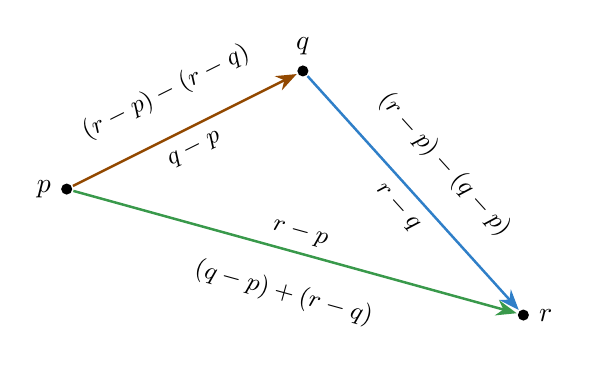
\begin{tikzpicture}
  \coordinate (p) at (0,0); \coordinate (q) at (3.0,1.5); \coordinate (r) at (5.8,-1.6);
  \draw[disp,cA] (p) -- node[lab,below]{$q-p$} node[lab,above=7pt]{$(r-p)-(r-q)$} (q);
  \draw[disp,cB] (q) -- node[lab,below]{$r-q$} node[lab,above=7pt]{$(r-p)-(q-p)$} (r);
  \draw[disp,cC] (p) -- node[lab,above]{$r-p$} node[lab,below=7pt]{$(q-p)+(r-q)$} (r);
  \foreach \x/\pos in {p/left,q/above,r/right} \node[pt,label=\pos:$\x$] at (\x) {};
\end{tikzpicture}
\end{document}
